\documentclass[12pt]{article}
\usepackage[T1]{fontenc}
\usepackage[T1]{polski}
\usepackage[utf8]{inputenc}
\newcommand{\BibTeX}{{\sc Bib}\TeX} 
\usepackage{graphicx}
\usepackage{amsfonts}
\usepackage{float}
\usepackage{amsmath}
\usepackage{subcaption}

\setlength{\textheight}{21cm}

\title{{\bf Zadanie nr 2 - Próbkowanie i kwantyzacja}\linebreak
Cyfrowe Przetwarzanie Sygnałów}
\author{Maciej Miazek 251589 \and Remigiusz Tomecki 251652}
\date{16.04.2026 r.} % Zaktualizowana data wedle postępów

\begin{document}
\clearpage\maketitle
\thispagestyle{empty}
\newpage
\setcounter{page}{1}
\section{Cel zadania}
Celem zadania 2 było poszerzenie dotychczasowo opracowanej aplikacji z zadania 1 o bloki konwersji analogowo-cyfrowej (A/C) oraz cyfrowo-analogowej (C/A). Zaimplementowane zostały metody próbkowania równomiernego, operacje rzutowania ciągłych wartości sygnału (kwantyzacja) wraz z technikami ograniczania błędu, oraz narzędzia do rekonstrukcji dziedziny ciągłej z analizą wyliczonego błędu i miar korelacji z oryginałem.\\

\section{Wstęp teoretyczny}
\subsection{Próbkowanie}

\subsubsection*{Próbkowanie równomierne (S1)}
Odtwarzanie dyskretnych wartości z ciągłego przebiegu analogowego. Proces przebiega z określoną częstotliwością $f_s$, która wyznacza nam okres próbkowania $T_s = \frac{1}{f_s}$. Otrzymane parametry zapisane są jako funkcja czasu w ciąg $x_n = x(n \cdot T_s)$. Kluczowym aspektem próbkowania jest zachowanie warunku określonego przez Twierdzenie Nyquista-Shannona ($f_s \ge 2f_{max}$).

\subsection{Kwantyzacja}
Proces transformacji wartości próbkowanego sygnału z nieskończenie dokładnego podzbioru na z góry określoną, dyskretną i uwarunkowaną limitami pamięciowymi mapę poziomów. Koncepcja opiera się na przybliżaniu, narzucając nieliniowy szum zwany szumem kwantyzacji.

\subsubsection*{Kwantyzacja równomierna z obcięciem (Q1)}
Algorytm odrzucający całą resztę wektora błędu (np. stosując zaokrąglenie w dół logiką \texttt{floor}). Wprowadza on systematyczny, stały defekt, celowo zaniżając zawsze wartość rekonstruowaną bez oceny odchylenia błędu.

\subsubsection*{Kwantyzacja równomierna z zaokrąglaniem (Q2)}
Matematyczne dopasowywanie (np. w standardzie logicznym \texttt{round}) zrekonstruowanej wartości do szczebla oddalonego na mapie bitowej o najkrótszy wektor błędu bezwzględnego. Wymusza centryzację błędu wokół naturalnej linii analogowej sygnału.

\subsection{Rekonstrukcja sygnału}
Kolejny krok toru przetwarzania, stanowiący odpowiedź konwerterów C/A - proces powrotu przebiegów dyskretnych przed oczy słuchacza do postaci ciągłej.

\subsubsection*{Ekstrapolacja zerowego rzędu (ZOH - R1)}
Najprostsza metoda pamięci stałej. Ustawienie analogowego woltażu na stałym poziomie (zamrożenie stanu) i utrzymanie go do momentu odebrania nowej próbki, przez co fizyczny kształt obrazuje typową krzywą trzymaną, czyli potocznie tzw. "schodki".

\subsubsection*{Interpolacja pierwszego rzędu (FOH - R2)}
Model operujący na zasadach ekstrapolatora wykorzystującego matematyczny styk obu sąsiadujących, bieżących próbek, wymuszający proste liniowe połączenie starych i nowych punktów po przekąsek.

\subsubsection*{Rekonstrukcja w oparciu o funkcję sinc (R3)}
Ideałem w rozumieniu warunku Nyquista. Sinc to interpolacyjna funkcja idealnego odtwarzającego filtru dolnoprzepustowego wygładzającego strome oploty, dająca gładkie krzywe po wyjściu z bufora: $sinc(x) = \frac{\sin(\pi x)}{\pi x}$.

\subsection{Miary podobieństwa}
Obliczenia parametrów pozwalają nam jednoznacznie i obiektywnie ustalić utratę informacji po operacjach przetworników.

\subsubsection*{Błąd średniokwadratowy (MSE - C1)}
MSE to potężna metryka oceny utraconej informacji (mocy sygnału kwantyzacji ubocznej): 
$$MSE = \frac{1}{N} \sum (x_{oryg} - x_{ZOH})^2$$

\subsubsection*{Stosunek sygnał-szum (SNR - C2)}
Oparty na skali logarytmicznej wskaźnik uwydatniania informacji ukrytej - im wyższy parametr (w dB), tym lepiej ukryty jest szum względem zregenerowanego sygnału:
$$SNR = 10 \cdot \log_{10} \frac{\sum x_{oryg}^2}{MSE}$$

\subsubsection*{Szczytowy stosunek sygnał-szum (PSNR - C3)}
Wrażliwa definicja badająca graniczny rzut maksymalnego wychylenia odchylonego od miary zniekształcenia:
$$PSNR = 10 \cdot \log_{10} \frac{MAX^2}{MSE}$$

\subsubsection*{Maksymalna różnica (MD - C4) i ENOB}
Miara określająca najwyższy pojedynczy uchwycony wektor dystansu szumu od uchybu naturalnej sinusoidy. Wyznacza się z niej po badaniu często również zastępczą liczbę działających bitów (ENOB: Effective Number Of Bits).


\section{Opis implementacji}
Aplikacja jest modularnie zintegrowana w Pythonie za pomocą \verb|Tkinter| ze sprawną biblioteką matematyczną \verb|Numpy| do odtwarzania buforów Sinc, z dodaną nową klasą z bloku konwersji \verb|KonwerterSygnalu|. Wynik przetwarzany jest asynchronicznie przez backendowe zaplecze układające podwójną osie (\textit{subplots}) za pomocą obiektowych metod \verb|FigureCanvasTkAgg|.


\section{Eksperymenty i wyniki}
W części tej analizujemy różnicę między sygnałem bazowym, a sygnałem po przejściu procesów wygenerowanych przetwornikiem.
%%%%%%%%%%%%%%%%%%%%%%%%%%%%%%%%%%%%%%%%%%%%%%%%%%%%%%%%%%%%%%%%%%%%%%%%%%%%%%%%%%%%%%%%%%%%%%%%%%%%%%%%%%%%%%%%%
% PODROZDZIAŁ PT. EKSPERYMENT NR 1
%%%%%%%%%%%%%%%%%%%%%%%%%%%%%%%%%%%%%%%%%%%%%%%%%%%%%%%%%%%%%%%%%%%%%%%%%%%%%%%%%%%%%%%%%%%%%%%%%%%%%%%%%%%%%%%%%

\newpage
\subsection{Wpływ częstotliwości próbkowania na rekonstrukcję w świetle Twierdzenia Nyquista}
Celem tego eksperymentu jest zaobserwowanie wpływu parametru $f_{probkowania}$ na odzyskaną i interpolowaną wartość częstotliwościową. 

\subsubsection{Założenia i Przebieg}
Generujemy oryginalny sygnał na przykład Sinusoidalny, a następnie drastycznie zmniejszamy $f_{sample}$ wokół niebezpiecznych granic pasma Nyquista doprowadzając do aliasingu. Dokonujemy na wykresie rekonstrukcji idealnej typu $Sinc$ i analizujemy logikę powstałych "odbić" (tzw. \textit{aliasing}). Oczekuje się spadków \textbf{SNR}.

\subsubsection{Rezultat}
\begin{table}[H]
    \centering
    \begin{tabular}{|c|c|c|c|c|}
    \hline
        \textbf{Częstotliwość próbkowania $f_{sample}$} & \textbf{1000 Hz} & \textbf{250 Hz} & \textbf{150 Hz} & \textbf{45 Hz} \\ \hline
        Błąd średniokwadratowy (MSE) & 0.000000 & 0.000924 & 1.104151 & 1.054363 \\ \hline
        Stosunek sygnał-szum (SNR) [dB] & 279.62 & 27.33 & -3.44 & -3.24 \\ \hline
        Szczytowy SNR (PSNR) [dB] & 282.42 & 30.13 & -0.65 & -0.45 \\ \hline
        Maksymalna Różnica (MD) & 0.000000 & 0.304146 & 1.938201 & 2.063781  \\ \hline
    \end{tabular}
    \caption{Tabela metryk błędu w zależności od zagęszczenia siatki Nyquista ($f_s$)}
\end{table}

\begin{figure}[H]
    \centering
    \begin{subfigure}{0.48\textwidth}
        \centering
        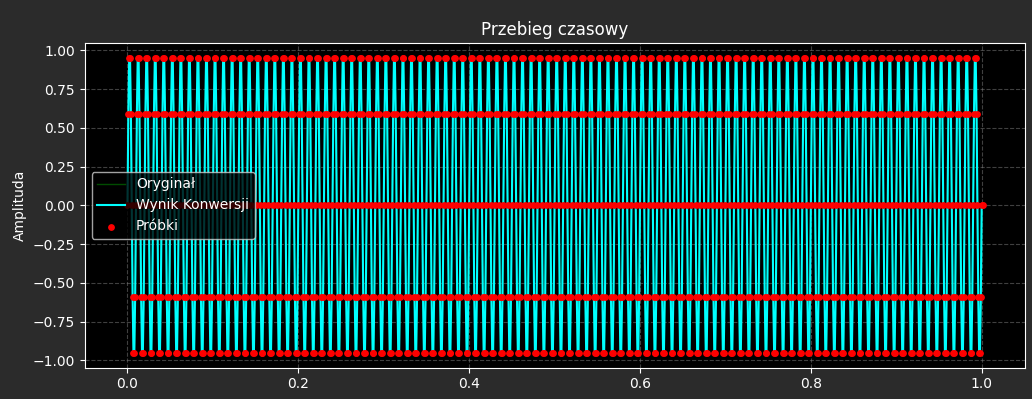
\includegraphics[width=\linewidth]{ex1/fs1000.png}
        \caption{Prawidłowe próbkowanie nadpróbkowaniem ($1000\text{Hz}$)}
    \end{subfigure}
    \hfill
    \begin{subfigure}{0.48\textwidth}
        \centering
        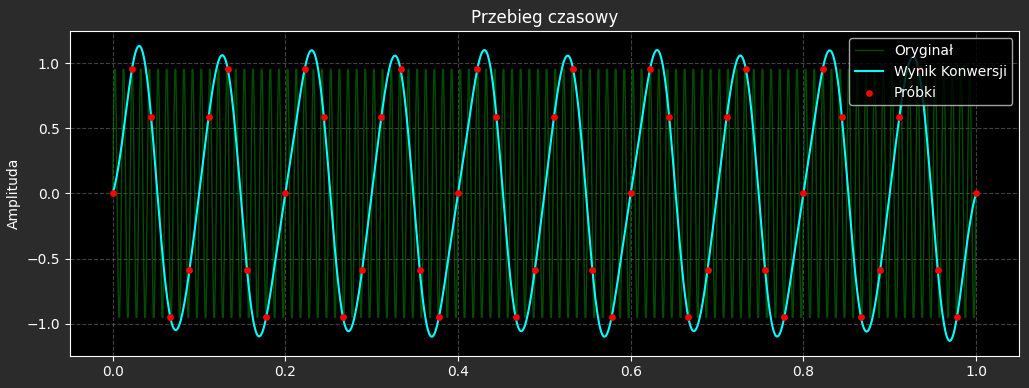
\includegraphics[width=\linewidth]{ex1/fs45.png}
        \caption{Zjawisko pełnego Aliasingu ($45\text{Hz}$)}
    \end{subfigure}
    \caption{Wizualizacja utraty zjawiska okresowego w dziedzinie ciągłej przy Sinc}
\end{figure}


%%%%%%%%%%%%%%%%%%%%%%%%%%%%%%%%%%%%%%%%%%%%%%%%%%%%%%%%%%%%%%%%%%%%%%%%%%%%%%%%%%%%%%%%%%%%%%%%%%%%%%%%%%%%%%%%%
% PODROZDZIAŁ PT. EKSPERYMENT NR 2
%%%%%%%%%%%%%%%%%%%%%%%%%%%%%%%%%%%%%%%%%%%%%%%%%%%%%%%%%%%%%%%%%%%%%%%%%%%%%%%%%%%%%%%%%%%%%%%%%%%%%%%%%%%%%%%%%

\newpage
\subsection{Analiza wpływu rozmiaru bitowego na wielkość i zjawisko dystansu skwantowanego szumu}
Celem tego eksperymentu była kwantyfikacja poziomu błędów po przejściu układów rejestru i ucięcia algorytmami floor/round.

\subsubsection{Założenia i Przebieg}
Bierzemy na warsztat klasyczny zestaw ciągły używając do niego kwantyzacji z Zaokrągleniem, badając poziomy i szczebelki w zależności od przypiętych bitów ($1, 2, 4 i 8 b$). Obserwujemy odczyty Effective Number Of Bits (ENOB)

\subsubsection{Rezultat}
\begin{table}[H]
    \centering
    \begin{tabular}{|c|c|c|c|}
    \hline
        \textbf{Zadeklarowane Bity} & \textbf{SNR [dB]} & \textbf{Wyliczony ENOB [bit]} & \textbf{Wyliczone MD} \\ \hline
        \textbf{2} & 12.21 & 1.7354 & 3.333333 \\ \hline
        \textbf{4} & 25.66 & 3.9703 & 0.666667 \\ \hline
        \textbf{8} & 49.95 & 8.0056 & 0.039216 \\ \hline
    \end{tabular}
    \caption{Odchylenia systemu ucinania w zależności od rozdzielczości rejestru zadanego przez użytkownika}
\end{table}

\begin{figure}[H]
    \centering
    \begin{subfigure}{0.48\textwidth}
        \centering
        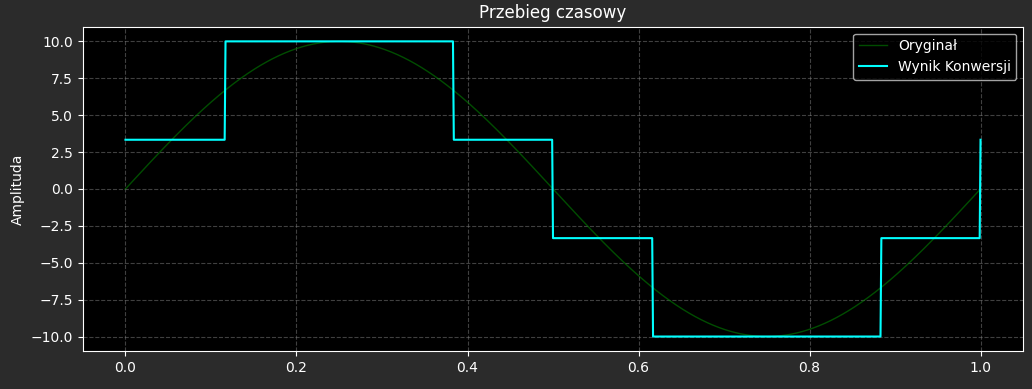
\includegraphics[width=\linewidth]{ex2/b2.png}
        \caption{Kwantyzacja: 2 bity}
    \end{subfigure}
    \hfill
    \begin{subfigure}{0.48\textwidth}
        \centering
        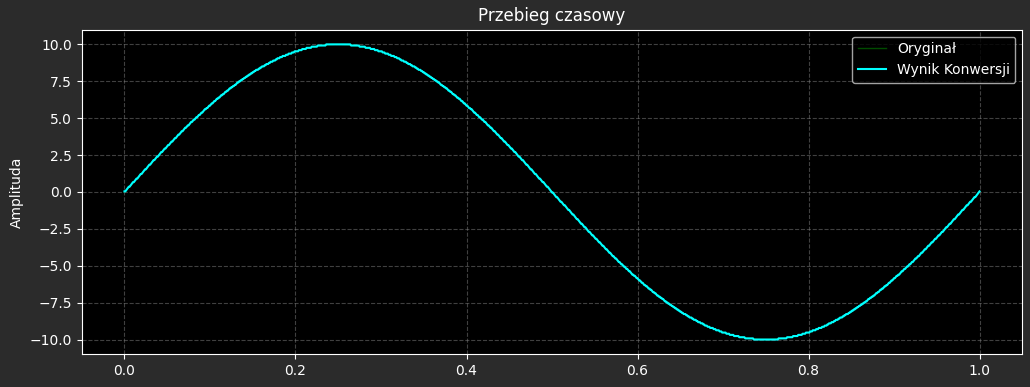
\includegraphics[width=\linewidth]{ex2/b8.png}
        \caption{Kwantyzacja: 8 bitów}
    \end{subfigure}
    \caption{Wizualizacja ograniczenia rozdzielczości pionowej kwantyzatora na wykresach}
\end{figure}

Z powyższej tabeli oraz badanych przebiegów w oknie histogramów można wyraźnie potwierdzić powiązanie matematyki kwantyzacji - szum rośnie nieliniowo proporcjonalnie do wykładniczych bloków bitowych, pozostawiając mniejsze logarytmiczne SNRy.


\newpage
\section{Wnioski}
Twierdzenie Kotielnikowa-Shannona w istocie określa minimalną barierę przejścia dziedziny C/A – sprowadzenie poziomu próbkowania poniżej zadeklarowanych $2f_{max}$ zawsze prowadziło do bezpowrotnej utraty bazy fizycznej przebiegów po nałożeniu rekonstrukcji na oś X.\\
Sklasyfikowaliśmy wyższość interpolacji pierwszego rzędu względem brutalnego blokowania ekstrapolacją ZOH, aczkolwiek pełen obiektyw zapewniła niefizyczna bariera rekonstrukcji Sinc, minimalizująca średniobłąd (MD) do zupełnych minimów pomijając tylko asymetrycznie niefortunne krawędzie buforów ramki aplikacyjnej.\\
System \texttt{KonwerterSygnalu} sprawdził się idealnie w demonstracji jak dużą zawiłość wyznacza obiektywne szacowanie sygnału do szumu (SNR, PSNR i ENOB).

\end{document}
